Computational campaigns for drug discovery require sizable compute resources
both in terms of scale and allocation. Typically, a computational campaign
explores a large number of drug candidates by running several workflows
multiple times, each requiring thousands of concurrent simulations. Before
embarking on a drug campaign that will utilize 150 million core hours on NCSA
Blue Waters, we perform experiments to characterize the weak and strong
scaling performance of HTBAC and its overheads on Blue Waters. We validate
the results of the free energy calculations produced using HTBAC by comparing
them to results that are already available in referenced literature.

Given that protocols like TIES are more computationally demanding than
protocols like ESMACS, it is paramount to use resource efficiently,
especially for campaigns that have a predefined computational budget. As
described in Sections~\ref{sec:science-drivers} and~\ref{sec:htbac}, adaptive
simulation methods have the potential for higher computational efficiency
when compared to non-adaptive simulation methods. Specifically, adaptive
simulation methods can reduce the number of simulations for each lead
candidate without a loss in free energy accuracy and with a lower
computational load. Further, given a defined number of resources, adaptive
methods can also increase computational efficiency by improving the rate of
statistical convergence and thereby reducing the time to solution.

Specifying, coordinating and executing adaptive simulation methods requires
middleware supporting runtime decisions. As seen in Section~\ref{sec:htbac},
HTBAC has been designed to enable decisions based on intermediate runtime
results. These results are evaluated to determine a redistribution of
resource to better support the execution of new simulations. We use HTBAC to
perform experiments about adaptivity, comparing and characterizing resource
efficiency with non-adaptive simulation methods.

% - Weak Scalability Design : Keep Pipeline of Ensembles to show barrier
%   needed in S5 and S6.
% - Performance, generality with weak scaling (agnostic to kernel) Added
%   functionality (do not speak about binding adaptivity to performance or
%   generality).
% - In use case: add in why TIES is challenging, and why adaptivity is
%   challenging.

% \mtnote{General note. \\
%         - Currently, this section is a merge of two distinct contributions.
%           These need to be better merged. For example, we should consider
%           whether (i) the description of the adaptive experiments should be
%           moved to the first subsection ``Experimental Setup''; (ii) Table 1
%           should be extended to include the adaptive/nonadaptive properties;
%           (iii) the discussion of the results should have a uniform
%           argumentative format; etc.\\
%         - The structure of the section should be revise making the division
%           in subsections consistent and changing/refining their naming.\\
%         - A.0,1,2 require major rewriting of the text and the writing of
%           relevant portions of new text. This includes: (i) eliminating
%           redundant (copied) text; (ii) Eliminating or referencing text
%           copied from other publications; (iii) reorganize the argumentation
%           following the other general note left in the comments and better
%           separating the experimental variables (especially including
%           adaptive/nonadaptive) properties; (iv) adding plots (even if with
%           incomplete results) and writing an actual analysis of the results
%           for each plot.}


% \jdnote{Revisions: \\ 
%         - Rewrote experimental setup by starting with motivation and
%           explaining overview of experiments
%         - Appended all experiments to table
%         - Created subsections for weak scaling, strong scaling, validation,
%           adaptive experiments
%         - Added plots (some are incomplete) and rearranged analysis
%         - Kristof added his data for adaptive experiments and
%           wrote results 
%         - Strong scaling subsection still waiting on data from ESMACS
%         - For now, removed anything related to Titan}

% \jdnote{should we mention anything about exascale?}\mtnote{I would not but
% I would quantify the scale at which we need to run. As it stands, this
% sentence appears too generic too me.} \jdnote{mentioned lower bound on
% concurrent number of simulations}

% \mtnote{what does this mean? We cited the results already in the paper?
% These results are published?}
% \mtnote{This sentence does not read well to me. I would refine, depending
% on the answer to the previous comment}.
% \jdnote{I meant to say we validate our free energy calculation results from
% this paper with known results . Does it make more sense now?}

% \mtnote{Grammar: more than?}\jdnote{more than ESMACS}
% \mtnote{Methods for? Maybe `simulation methods'?}

% \mtnote{simulation?}
% \mtnote{simulation?} 
 
% \mtnote{Note: experiments are not adaptive, they are about adaptive
% simulation methods. Analogously, experiments are not compared to
% non-adaptive experiments but they (should) offer comparable data about both
% types of methods.} \mtnote{Note: I rewrote the whole paragraph. The
% previous version was compressed and ``left too much in the authors'
% pens''.}

% ---------------------------------------------------------------------------
\subsection{Experiment Setup}\label{ssec:exp_design}

Table~\ref{tab:experiments} shows 7 experiments we designed to characterize
the behavior of HTBAC on Blue Waters. Each experiment executes the ESMACS
and/or TIES protocol for different physical systems. Experiments 1--5 use the
BRD4 physical systems provided by GlaxoSmithKline, while experiments 6 and 7
utilize the PTP1B, MC1, and TYK2 physical systems which are a diverse set of
proteins.

\begin{table*}
    \caption{Parameters of scalability and adaptivity experiments.}
    \label{tab:experiments}
    \centering
    \resizebox{\textwidth}{!}{
    \begin{tabular}{l            % Experiment ID
                    l            % experiment type
                    l            % physical system 
    %                l            % CI
                    l            % protocol type
                    l            % number of protocols
                    l            % total cores
                    }
    %
    \toprule
    %
    \B{ID}                            &  % Experiment ID
    \B{Type of Experiment}            &  % experiment type
    \B{Physical System(s)}            &  % physical system
    % \B{Computing Infrastructure (CI)} &  % CI
    \B{Protocol(s)}                   &  % protocol type
    \B{No. Protocol(s)}               &  % number of protocols
    \B{Total Cores}                   \\ % total cores
    %
    \midrule
    %
    \B{1}                             &  % Experiment ID
    Weak scaling                      &  % experiment type
    BRD4                              &  % physical system
    % Blue Waters                       &  % CI
    ESMACS                            &  % protocol type
    (2, 4, 8, 16)                     &  % number of protocols
    1600, 3200, 6400                  \\ % total cores
    % 
    \B{2}                             &  % Experiment ID
    Weak scaling                      &  % experiment type
    BRD4                              &  % physical system
    % Blue Waters                       &  % CI
    TIES                              &  % protocol type
    (2, 4, 8)                         &  % number of protocols
    4160, 8320, 16640                 \\ % total cores
    %
    \B{3}                             &  % Experiment ID
    Weak scaling                      &  % experiment type
    BRD4                              &  % physical system
    % Blue Waters                       &  % CI
    ESMACS + TIES                     &  % protocol type
    (2, 4, 8)                         &  % number of protocols
    5280, 10560, 21120                \\ % total cores
    %
    \B{4}                             &  % Experiment ID
    Strong scaling                    &  % experiment type
    BRD4                              &  % physical system
    % Blue Waters                       &  % CI
    TIES                              &  % protocol type
    (8, 8, 8)                         &  % number of protocols
    16640, 8320, 4160                 \\ % total cores
    %
    \B{5}                             &  % Experiment ID
    Strong scaling                    &  % experiment type
    BRD4                              &  % physical system
    % Blue Waters                       &. % CI
    ESMACS                            &  % protocol type
    (16, 16, 16)                      &  % number of protocols
    6400, 3200, 1600                  \\ % total cores
    %
    \B{6}                             &  % Experiment ID
    Non-adaptivity                    &  % experiment type
    PTP1B, MC1, TYK2                  &  % physical system
    % Blue Waters                       &  % CI
    TIES                              &  % protocol type
    (1, 1, 1)                         &  % number of protocols
    2080, 2080, 2080                  \\ % total cores
    %
    \B{7}                             &  % Experiment ID
    Adaptivity                        &  % experiment type
    PTP1B, MC1, TYK2                  &  % physical system
    % Blue Waters                       &  % CI
    TIES                              &  % protocol type
    (1, 1, 1)                         &  % number of protocols
    2080, 2080, 2080                  \\ % total cores
    %
    \bottomrule
    %
    \end{tabular}
    }
\up{}
\end{table*}

Experiment 1 and 2 measure the weak scalability of HTBAC using multiple
instances of the ESMACS (experiment 1) and TIES (experiment 2) protocol.
Experiments 3 uses both the TIES and ESMACS protocols, characterizing the
weak scaling of heterogeneous protocol executions. Experiments 4 and 5
measure the strong scalability of HTBAC using a fix number of instances of
the ESMACS (experiment 4) or TIES (experiment 5) protocol. Experiments 6 and
7 characterize nonadaptive and adaptive simulation methods using the TIES
protocol.

In each weak scaling experiment (1--3), we keep the ratio between resources
allocated and protocol instances constant. Consistently, for each experiment
we progressively increase both the number of cores (i.e., measure of
resource) and the number of protocol instances by a factor of 2. In each
strong scaling experiment (4--5), we change the ratio between resources
allocated and the number of protocol instances. For each experiment, we fix
the number of protocol instances and reduce the number of cores by a factor
of 2.

Weak scaling experiments provide insight into the size of the workload that
can be executed in a given amount of time, while strong scaling experiments
show how the time duration of the workload scales when adding resources. For
all the weak and strong scaling experiments we characterize the overheads of
HTBAC, EnTK and RP, and we show an approximation of the time taken by the
resources to become available. This offers insight about the impact of HTBAC
and its middleware on the time to completion of each workload.

For weak and strong scaling experiments, we reduced the number of time-steps
of the protocols and omitted the analysis steps $S5$ and $S6$ of their
workflows (Figure~\ref{fig:ties_esmacs_application}). These simplifications
are consistent with characterizing scalability performance instead of
simulation duration. For the experiments 1--5 we used the following
time-steps: $S1=1000$; $S2=5000$; $S3=5000$; and $S4=50000$.

Experiments 6 and 7 compare the the accuracy and time to solution of
nonadaptive and adaptive simulation methods. For the nonadaptive simulation
method of Experiment 6 we use 13 preassigned and approximated $\lambda$
windows, consistent with the value reported in Ref.~\cite{Bhati2017}. In this
way, we produce 65 concurrent simulations for stages $S1$--$S4$ of the TIES
workflow (Figure~\ref{fig:ties_esmacs_application}). The production
simulation stage $S4$ executes each simulation for 4ns. Stage $S5$ consists
of 5 analysis tasks which aggregate the simulation results of $S4$. The
global analysis stage $S6$ contains a single task that aggregates the results
from $S5$.

In the adaptive workflow~\ref{fig:adaptive_ties}, we initialize the TIES
protocol with 3 $\lambda$ windows, obtaining 15 replicas. We separate stage
$S4$ of each TIES replica into 4 sub-stages. Each sub-stage runs a 1ns
simulation, followed by an adaptive quadratures analysis which estimates free
energy errors with respect to each interval of two $\lambda$ values. We
evaluate the total number of $\lambda$ windows as determined by the adaptive
quadrature results in order to measure the differences in time duration
between adaptive and non-adaptive methods as well as the differences in
accuracy.\mtnote{I had to simply this paragraph a lot. Please check whether I
omitted some essential detail or got the algorithm wrong.}
\jdnote{it works}

\begin{figure}
  \centering
  \includegraphics[width=\columnwidth]{figures/Adaptive_TIES.pdf}
  \caption{Adaptive workflow for TIES. After equilibrating 3 initial
  $\lambda$, the first production stage starts. This is followed by analysis
  at every $\lambda$ interval, to decide whether to add a new window in
  between. In our implementation, the production-analysis cycle is repeated
  for 4 production steps, not shown here.}
\label{fig:adaptive_TIES}
\end{figure}

% \mtnote{For quality reasons, it would be better to use figures in pdf
%   format.}\jdnote{addressed}.

For Experiment 6, we assigned the following simulation time-steps: $S1=3000$;
$S2=50000$; $S3=50000$; and $S4=2000000$. The adaptive simulation method of
Experiment 7 uses the same simulation time-steps, apart from $S4$ which is
divided into 4 sub-stages of 500000 time-steps each. 

% \jdnote{should we
% mention relationship between ns and time-steps?}

We performed all the experiments on Blue Waters, a 26868 node Cray XE6/XK6
SuperComputer with peak performance of 13.3 petaFLOPS managed by NCSA. We
initiated the experiments from a virtual machine outside NCSA. In this way,
we did not run any persistent process on the NCSA login node, consistent with
NCSA usage policies. We used HTBAC 0.1, EnTK 0.6, and RP 0.47 and the same
versions of the \texttt{NAMD-MPI} MD kernel, compiled according to the
capabilities of each environment and of \texttt{NAMD} itself, and launched
via the \texttt{aprun} command. For the analysis stages in the TIES protocol
we used \texttt{AmberTools}.

NCSA sets a system policy on the maximum number of processes that
\texttt{aprun} can spawn, limiting the number of concurrent tasks we can
execute on Blue Waters to approximately 450. During the execution of
Experiment 2, we observed failing tasks once we scale up to 8 TIES protocol
instances, which is equivalent to 520 concurrent tasks. In a trial of 10
repetitions at this scale, we observed an average of 70 failing tasks, with a
standard deviation of 6.67, and range of 59 to 83 tasks. Given that we only
ran a small number of trials, more data would be required to properly model
the distribution type of these results.

NCSA allows to run only one MPI application for each compute node. As a
consequence, we had to run each MD simulation with 32 cores (i.e., one full
compute node) even if our performance measurement of \texttt{NAMD} on Blue
Waters indicated that 16 cores would offer the best trade-off between
computing time and communication overhead.

% \jdnote{Should we include the scalability plot of
% a single NAMD task using aprun?}

% \mtnote{The following paragraphs are disconnected from the previous ones.
% We need a `joining' paragraph starting from something like: ``We designed n
% experiments\ldots We used m protocols\ldots See Table o\ldots''. Moved a
% paragraph here as a starting point.}\jdnote{provided ``segway"}

% Experiment 2 measures weak scaling performance of ESMACS at higher scales,
% using ORNL Titan.
% \mtnote{Would it be better to describe weak scaling in terms of solution
% time, number of resources and problem size, as done in the following
% paragraph?}\jdnote{moved to previous para when first introducing weak
% scaling}

% of the protocols \mtnote{which protocols? So far we wrote about methods
% (but we did not specify what type of methods are we referring to)}
% \jdnote{Does the modified description of the protocol types in the earlier
% paragraph give enough insight?} \mtnote{required by what/whom? ``keeping
% the number of pipelines fixed at the number required by \ldots'' or
% something like that?} \jdnote{I've changed this description of ws, do this
% sentence and the next suffice?}

% By design of each protocol, an increase in the number of instances means an
% increase in the number of pipelines. Further, \jdnote{mention the
% relationship between protocols and pipelines in section IV.}

% \mtnote{property of? I would replace with: ``weak scaling provides
% insight\ldots''} provides insight

% Next, we measure strong scaling performance of the ESMACS and TIES
% protocols in experiments 4 and 5, respectively, by fixing the number of
% protocol instances, but reducing the cores by a factor of 2 in each run.

% \mtnote{which ones?} by fixing the workload i.e. \mtnote{Grammar: please be
% careful about the use of `i.e.' as explained in my previous set of
% comments}
% \mtnote{Why do we need the `i.e.' at all? What does `workload' add?
% ``\ldots by fixing the number of pipelines of each protocol and reducing
% \ldots''}
% \jdnote{also changed this description of ss.}

% the number of cores by a factor of 2 in each run.

% \mtnote{what does `timing' mean in this context? Duration? }
% \jdnote{will be defined in section IV}\mtnote{we will define
% `what'?}\jdnote{ignore earlier comment, the correct phrasing is time
% duration of the workload, but I am not sure if this causes
% confusion}\jdnote{ also workload will be defined in Section IV}

% \jdnote{expecting linear speedup, and expect fixed overheads}\mtnote{is
% this comment about text that still needs to be written? If so, I would not
% mention expectations of results in the design section.}

% \mtnote{of?}\jdnote{addressed}

% Experiments 4 measures the strong scaling performance of ESMACS while
% experiment 5 repeats the same strong scaling experiment using the TIES
% protocol.

% \mtnote{This is a placeholder for an actual paragraph: note how the
% previous paragraphs have a structure based on numbering experiments (and
% referring them to the table via references that are still missing), while
% this and the following paragraphs do not use the same structure. Please
% expand as needed and note that a section is not `ready' until this kind of
% uniformity is not achieved.}\jdnote{I've added experimental design of
% adaptive/nonadaptive methods.}

% Keep iterating on the next two paragraphs to get the right description from
% Kristof

% We perform the experiments for the nonadaptive (experiment 6) and adaptive
% (experiment 7) simulation methods with the same number of cores and
% simulation duration (Table~\ref{tab:experiments}). By fixing these
% parameters, we enable the comparison between the accuracy and time to
% solution of the two methods.

% By design of the nonadaptive TIES workflow
% (Figure~\ref{fig:ties_esmacs_application}), each $\lambda$ window creates a
% new simulation condition that must be replicated. TIES requires 5 replicas
% per $\lambda$, thereby producing $\lambda \times 5$ or simulations.

% \mtnote{Reference table and exp number}
% \jdnote{addressed in this and previous sentence}
% \mtnote{Reference table with S*}
% \jdnote{the ref to Figure~\ref{fig:ties_esmacs_application} already points
% to the description of S*, no?}
% \mtnote{Grammar: no spaces before and after dashes}
% \jdnote{noted}
% \jdnote{reworded this paragraph}

% \mtnote{Grammar: it is not clear to what this `this' refers to} produces a
% total of 65 concurrent simulations for stages $S1$--$S4$ \mtnote{Reference
% table with S*} \mtnote{Grammar: no spaces before and after
% dashes}\jdnote{noted}. The production simulation stage $S4$ executes each
% simulation for 4ns. The analysis stage $S5$ assigns 5 analysis tasks which
% aggregate simulation results of $S4$ with respect to each replica. The
% global analysis stage $S6$ contains a single task that aggregates the
% results from $S5$.

% \mtnote{different from what?}\jdnote{changed}

% The estimation of the error determines whether
% \mtnote{Grammar: as already commented in the previous draft, `whether'
% implies already `or not'.\jdnote{noted} Adding it is
% redundant.}\jdnote{noted} to spawn additional $\lambda$ windows. If the
% error estimate in a certain interval is higher than the acceptable
% threshold, a new $\lambda$ window is assigned halfway between the interval.
% If the critical threshold is reached, we have reached convergence and the
% application stops; else, current simulations continue executing and new
% simulations begin executing based on newly generated $\lambda$ windows.

% The estimation computation \mtnote{This is too compressed. In itself,
% `estimation computation' means little. The reader has to go back to the
% previous paragraph to understand what those two words refer to. `We compute
% the free energy errors\ldots'?} is captured \mtnote{`captured' is
% metaphorical. Metaphors should be avoided when writing science. Also, the
% sentence is passive and also this should be avoided in scientific writing}
% as a single stage \mtnote{Does the reader know what a stage is?} containing
% a single task. By design of the adaptive quadrature algorithm \mtnote{where
% this algorithm is used? Does the reader know about it?}, the number of
% additional $\lambda$ windows will vary across candidates, which will impact
% the number of simulation-analysis iterations. \mtnote{And\ldots We are
% missing an explanation of why this is important from an experimental design
% point of view. Maybe because it changes the number of tasks?}
% \jdnote{will call this something else}.\jdnote{check with Kristof on the
% local and global analysis that happen for nonadaptive}

% \mtnote{Note: paragraphs like this indicate lack of iteration before
% releasing the manuscript for review. Too much is assumed, too little is
% converted from thoughts to written form. How the academic writing process
% works: Before releasing the manuscript for review, the author goes back and
% forth across the manuscript multiple times. Progressively, each paragraph
% is iterated until it is grammatically correct and it stands on its own
% content-wise. When a manuscript is received for review, the reviewer focus
% on the content of each paragraph and section, assessing their completeness
% and conceptual/formal correctness. Each grammatical error, each
% inconsistency or missing detail distracts the reviewer impeding her
% work.}\jdnote{I've removed the previous paragraph that gave trouble and
% updated the experimental setup of the adaptive and non-adaptive methods.}

% This procedure is repeated until convergence, at which point all concurrent
% simulation are terminated. We define convergence as the point in the
% production-analysis loop at which a desired error threshold is reached.

% When one protocol has converged whilst another has not, we can shift
% computational resources to favor simulations that require additional
% resources.

% individual\mtnote{I am not sure I understand what individual means in this
% context}

% strong scaling performance of ESMACS and TIES on Blue Waters. We fix the
% number of protocols and vary the amount of resources in order to produce
% generations

% \mtnote{The reader will struggle to understand what `generations' means in
% this context.} of execution.
% \mtnote{Two sizable paragraphs to describe weak scaling, four lines to
% describe strong scaling? I would expand.}

% \mtnote{This sentence seems to suggest that we run our experiments on a
% virtual machine. I know what you mean but the average reader has no idea
% about the capabilities of our middleware and the policies of not executing
% persistent processes on the head node of Blue Waters.}
% \jdnote{Can we omit this sentence?}

% and the Titan ones from an ORNL login node. as Blue Waters does not permit
% executing applications directly on the login node. The ORNL Titan
% experiments had instead to be performed from an ORNL login node.

% The minimization tasks of $S1$ to 1000 simulation time steps, while the
% equilibration tasks in $S2$ and $S3$ are \mtnote{Grammar: inconsistent
% tense. `Were' or `assign'} assigned 5000. The MD simulation tasks in $S4$
% are assigned 50,000 steps.

% \mtnote{when/why a simulation task is `production'? I am not sure I
% understand what that means}\jdnote{removed production for weak/strong.
% Production applies to adaptive/nonadaptive which need to show the
% production scale timesteps i.e. 2 or 3M}

% while on Titan a non-MPI, multi-core NAMD engine. On Titan we compiled NAMD
% with CUDA for the ESMACS experiments, and with OpenMP for the for TIES ones
% as NAMD does not support alchemical perturbations execution on GPU.

% application launch method, which is the NCSA Blue Waters designated command
% for describing the application parameters and resource requirements
% \mtnote{does the reader know what is a launch method?} \jdnote{better?}
% \mtnote{Unfortunately not: https://bluewaters.ncsa.illinois.edu/using-aprun
% . Alternative: `We perform (or performed depending on what tense you will
% decide to use) all Blue Waters experiments using the \texttt{aprun} command
% to launch the MD simulations'}.
% \jdnote{noted and addressed.} During our scalability experiments we found
% two main limitations.
% \mtnote{this is too generic. Based on this paragraph, we found two main
% limitations. This is what we should therefore write.}

% \jdnote{I've changed this again because the limitation on the max no. of
% concurrent CUs is a system setting (similar to what we experienced
% first-hand on Titan), but it's not a technical limitation of APRUN.}

% Unfortunately, \texttt{aprun} has several \mtnote{this is too generic.
% Based on this paragraph, we found two main limitations. This is what we
% should therefore write.} limitations: First, the number of concurrent tasks
% execution is limited to \ldots. On average, during our experiments we were
% not able to execute more than 436 concurrent tasks.
% \mtnote{how do we know this average?}.
% \jdnote{would it make sense to show a bell curve of the distribution of
% failing units? I have 8 data points, but I can run more and include Mark's
% Cray paper?}
% \mtnote{Agreed. The comment was about saying that you observed this average
% while performing experiments. See how I rewrote the paragraph}.
% \jdnote{added the data for the failing units however including a
% distribution of this data is not meaningful as the sample size in the
% number of trials is very small. By looking at some histograms where I vary
% the bin size, it could be either Gaussian or multimodal distribution. Only
% more data will tell us for sure what kind of distribution we have.
% Moreover, Mark's Cray paper shows range of concurrent units using ORTE-LIB,
% so I will not reference this here.}

% \mtnote{this is metaphorical. Please change using a factual predicate.}
% \jdnote{changed the phrasing a bit}
% \mtnote{Note: I had to rewrite the paragraph because the current version
% was too unrefined. Please see the note above about the need to
% progressively refine each paragraph.}

% From our own scalability performance measurements of NAMD on Blue Waters,
% we observe the ideal cores per task to be 16, however Blue Waters does not
% permit running multiple MPI applications on the same node, hence each NAMD
% task requires a complete node to maintain concurrency.
% \mtnote{This needs to go before previous sentence as it explains why we use
% 32 cores for each NAMD executable. Note: it is not true that NAMD
% `requires' 32 cores as stated above.}\jdnote{moved here since this para
% discusses \texttt{aprun} limitations}

% In order to continue execution on higher scales \mtnote{Why do we need an
% higher scale?}, we perform higher scales \mtnote{I am not sure what
% `performing higher scales' means} on ORNL Titan, using the ORTE launch
% method \mtnote{Why don't we use ORTE on BW? The reader will probably know
% that they are similar machines}.

% The difference in platforms produces overheads \mtnote{Only overheads or
% also different execution time of NAMD---seeing the differences described in
% the previous paragraph} that can be captured by RTS \mtnote{does the reader
% know what a RTS is?} and are shown \mtnote{careful with the use of
% `demonstrate', especially in a scientific paper} in the figures
% \mtnote{which figures?} as "APRUN overhead" and "ORTE overhead"
% \mtnote{LaTeX requires different quotes}.

% For tasks pertaining to $S1$ -- $S4$ \mtnote{What are $S1$ and $S4$? LaTeX
% wants double dash without space to indicate a range}, while the analysis
% stage, $S5$ use AmberTools \mtnote{grammar: I am not able to parse this
% sentence}.

% For both adaptive and nonadaptive experiments \mtnote{the reader knows
% about Experiment 1-7, not about adaptive/nonadaptive ones},

% In the nonadaptive experiments,

% For the adaptive experiments, each substage
% \mtnote{What is a `substage'?} of $S4$ i.e. $S4.1$--$S4.4$ is assigned
% 50,000 steps.\mtnote{Why the difference is number of steps and why it is
% relevant?}

% HTBAC submits a resource request to EnTK, to which EnTK uses RP to acquire
% resources via a single pilot. Accordingly, we request the maximum number of
% cores required by the workload as the number of cores in a pilot.

% To characterize the weak scaling performance of TIES \mtnote{I am not sure
% I understand this sentence: For measuring the weak scaling performance of
% TIES?}
% \jdnote{better?}, we use between 4160 and 33280 cores as indicated in
% Figure~\ref{fig:weak_scaling_TIES} because the NAMD executable used in all
% tasks \mtnote{does the reader know what a task is in this context?}
% \jdnote{will be defined in Section IV} from $S1$-$S4$ require
% \mtnote{grammar: requires} a single node i.e. 32 cores per task, as
% mentioned earlier in the APRUN limitation.
% \mtnote{why?}\jdnote{32 cores/task addressed by earlier mention of aprun
% MPI limit}

% For strong scaling performance, we fix the number of protocol instances to
% 8 instances given that we experience failing concurrency of tasks when we
% scale the workload to 8 protocols.\mtnote{why 8?} We vary the amount of
% resources as shown in Figure~\ref{fig:strong_scaling_TIES} by showing
% reducing of resources by a factor of 2. \mtnote{Please expand indicating
% and justifying the the chosen amount of resources. Experiments can be
% design in many ways, we need not only to describe but also to justify why
% we choose a specific design for our experiments.}\jdnote{better?}

% For the TIES protocol, each pipeline \mtnote{does the reader know what a
% pipeline is?}\jdnote{will be address in Section IV} consists of six stages
% \mtnote{simulation stages?}. Each of the simulation stages contains a task
% for every unique ($\lambda$, replica) combination \mtnote{does the reader
% understand this?}\jdnote{will be addressed better in section IV}. In the
% non-adaptive workflow \mtnote{we never used `workflow'. Previously we used
% non-adaptive (written as `nonadaptive') experiment. Note that we did not
% introduce adaptive/nonadaptive experiments} scenario, the first 11
% $\lambda$ windows
% \mtnote{does the reader know what a lambda window is?} consist of the
% following values: $L$ is a vector with
% \begin{flalign} L &= \{ x_i: x_i\in[0,1]\; and\; x_{i+1} = x_i + \delta \},
% where\ \delta\ is\ 0.1. %&$$L=\{ x_i: x_i\in[0,1]\; and\; x_{i+1} = x_i +
% \delta \}$$%, where $\delta$ is $0.1$.
% \end{flalign}

% We append two additional values on both ends of $L$, completing 13
% $\lambda$ windows. Each $\lambda$ window consists of five replicas.
% Therefore there are a total of 65 tasks for every simulation stage
% \mtnote{depending on the previous sections of the paper, this `therefore'
% may have to be better explained to the reader}. The production simulations
% stage, $S4$ as described in figure~\ref{fig:pst}\mtnote{missing figure}
% executes a 4 ns simulation duration \mtnote{grammar: executes a simulation
% for 4 ns? a simulation with a 4 ns duration?}. The analysis stages of the
% protocol reduce the number of tasks \mtnote{Why/how?}. The first analysis
% task consists of five tasks where each task performs an aggregate analysis
% over all $\lambda$ windows for each replica. The second analysis stage
% consists of one task that aggregates the previous results and computes a
% single average across all replicas.

%----------------------------------------------------------------------------

\subsection{Characterization of Scalability Experiments}

We perform 5 experiments to characterize the overheads of HTBAC, EnTK and the 
runtime system, and \texttt{aprun} as a function of weak and strong scaling 
properties. We compare these overheads to the total execution time of all the 
tasks to assess their overall impact on the application duration. 
The durations we measure are defined as:

\begin{itemize}
    \item Task Execution Time: Time taken by the task executables to run on the 
    CI. 
    \item HTBAC Overhead: Time taken to process the application, instantiate the 
    components and subcomponents, translate protocols into pipelines for EnTK, 
    and validate resource descriptions. 
    \item EnTK and RP Overhead: Time taken by ensemble management system and the 
    runtime system to submit and manage the execution of tasks. 
    \item \texttt{aprun} Overhead: Time taken by \texttt{aprun} to schedule
    tasks on a set of compute nodes. 
\end{itemize} 

Total Time to Execution \(TTX\) measures only the aggregated execution time of 
all tasks' executables. 
\mtnote{TTX should measure only the aggregated time spent executing the
tasks' executables. All the rest should be part of RP overhead} 
\jdnote{
This sentence doesn't need to go in but I wanted to clarify a point: I would 
like to know if we should use TTX as TTX or something else like Task Execution Time. 
We have TTX measured by events: \texttt{cu-exec-start} and \texttt{cu-exec-stop}
, since \texttt{aprun} doesn't allow further scrutiny using events like 
\texttt{app-start} until \texttt{app-stop}. 
We use the term TTX internally, but maybe for this paper we should call it task 
execution time. TTX sounds like time to execution which could interpret the 
entire application, no?}

Once the runtime system relinquishes control flow to \texttt{aprun}, the 
precise times of when \texttt{aprun} schedules the task on the compute
nodes and when the MD kernel begins execution cannot be measured. Instead we 
approximate the \texttt{aprun} overhead by measuring the difference between 
TTX/Task Execution Duration and the total \texttt{NAMD} execution time, provided
by the \texttt{NAMD} output logs. 

% We characterize the execution time of all three applications \mtnote{which one?},
% \jdnote{given that I mention what each experiment entails earlier, can I keep 
% the application general and say all 3?} and overheads of HTBAC, EnTK, RP and 
% \texttt{aprun}. 

% \jdnote{Since we are showing overhead component separate, can we remove the
% total overhead calculation?}

% The total time to completion (TTC) of each application \mtnote{of what?} 
% \jdnote{per application} \mtnote{you see the difference produced by my 
% editing?} can be expressed as $TTC = TTX + T_{O}$ where Total Time to Execution 
% \(TTX\) measures only the aggregated execution time of all tasks' executables. 
% \mtnote{TTX should measure only the aggregated time spent executing the
% tasks' executables. All the rest should be part of RP overhead}\jdnote{for
% discussion with Matteo 06/04}\mtnote{I am afraid I do not understand this
% comment} 




% % $T_{O}$ equates to the total overheads produced by HTBAC, EnTK, and
% % RP: $$T_{O} = T_{O}\textsuperscript{HTBAC} + T_{O}\textsuperscript{EnTK} +
% % T_{O}\textsuperscript{RP}$$ 




% \mtnote{As defined, this formula seems to add
% twice part of the RP overheads.}
% \jdnote{I think I'm missing something: The RP
% overhead is what I get from the pilot duration logs. Not sure where I'm
% duplicating}
% % \mtnote{If TTX is more than just the aggregated execution time of
% % all the tasks' executable, then TTX and $T_{O}$ both contain part of RP
% % overhead.}

\subsection{Weak Scaling and Performance Characterization}

% \mtnote{Is this meant to be a subsubsection?}\jdnote{changed weak, strong
% and adaptive experiments \& results to subsections}

We investigate the weak scaling of HTBAC using three
applications \mtnote{which ones?}\jdnote{addressed}: Experiment 
1 using TIES-only, Experiment 2 using ESMACS-only, and Experiment 3 using
both TIES and ESMACS configurations. Each application uses a different protocol 
configuration with a number of instances determined by the 
number of concurrent executions supported by \texttt{aprun}. In each experiment, 
we increase the number of instances of the protocol configuration, 
proportionally to the amount of requested resources. 

Experiment 1 in Figure~\ref{fig:ws} (a) measures the weak scalability of HTBAC 
with the TIES protocol. Each instance of the TIES protocol contains a single 
pipeline with 4 stages and 65 concurrent tasks. We increase the number of 
instances linearly, between 2 and 8. When scaling to 8 protocol instances, we 
execute beyond the average limit of 450 concurrent tasks. 
Nevertheless, we include results at this scale to show HTBAC's performance 
capabilities in supporting higher orders of concurrent simulations. 

Experiment 2 in Figure~\ref{fig:ws} (b) measures weak scalability with the 
ESMACS protocol. We increase the number of instances linearly, between 2 and 16. 
Each ESMACS protocol contains 1 pipeline with 4 stages and 25
concurrent tasks \mtnote{Do we `increase the number of instances linearly,
between 2 and 8' also in experiment 2? If so, we should say that only once
for Experiment 1--3. If not, why?}\jdnote{addressed the scaling ranges, and 
explained why}. 

Experiment 3 in Figure~\ref{fig:ws} (c) measures weak scalability
with instances of both TIES and ESMACS protocols. Also in this case, we scale
the instances of both protocols linearly, between 2 and 8. Experiments 2 and 3 
show scalability ranges within the limit of the maximum number of concurrent 
tasks we can successfully execute on Blue Waters. For all weak
scaling experiments we use \mtnote{Grammar: conjugation}\jdnote{back to the 
present} physical systems from the \texttt{BRD4-GSK} library with the same 
number of atoms and similar chemical properties. The uniformity of these 
physical systems ensures a consistent workload that is insignificant to any 
variability in performance characterization. 
\jdnote{this is to say that the fluctuations in
execution times between data points are invariant to the physical
systems}\mtnote{Nice comment, I would edit it and put it in the text!}.
\jdnote{addressed}

% \mtnote{does the reader know what a task is in this context?} \jdnote{will
% be defined in Section IV}



% \mtnote{grammar: I do not understand the sentence after the `;'} given by
% the sum of the constituent overheads: $$T_{O} =
% T_{O}\textsuperscript{HTBAC} + T_{O}\textsuperscript{EnTK} +
% T_{O}\textsuperscript{RP}$$.

In all weak scaling experiments (Figure~\ref{fig:ws}) we
observe TTX showing ideal weak scaling behavior 

\mtnote{Please refine the previous sentence as it might not
say what I think you want to say: What does it mean that TTX is `within error
margin'? And how this relates to `ideal weak scaling behavior'? Maybe the
former applies to the latter instead of TTX?}. The error bars are calculated
using 3 trials per protocol instance measure.\mtnote{This might be consider
little without further explanation}

\dwwnote{The figure captions and legends don't appear to agree which axis 
applies to which measurement. Also the legend should be inside the plots.}

\begin{figure}
  \centering
    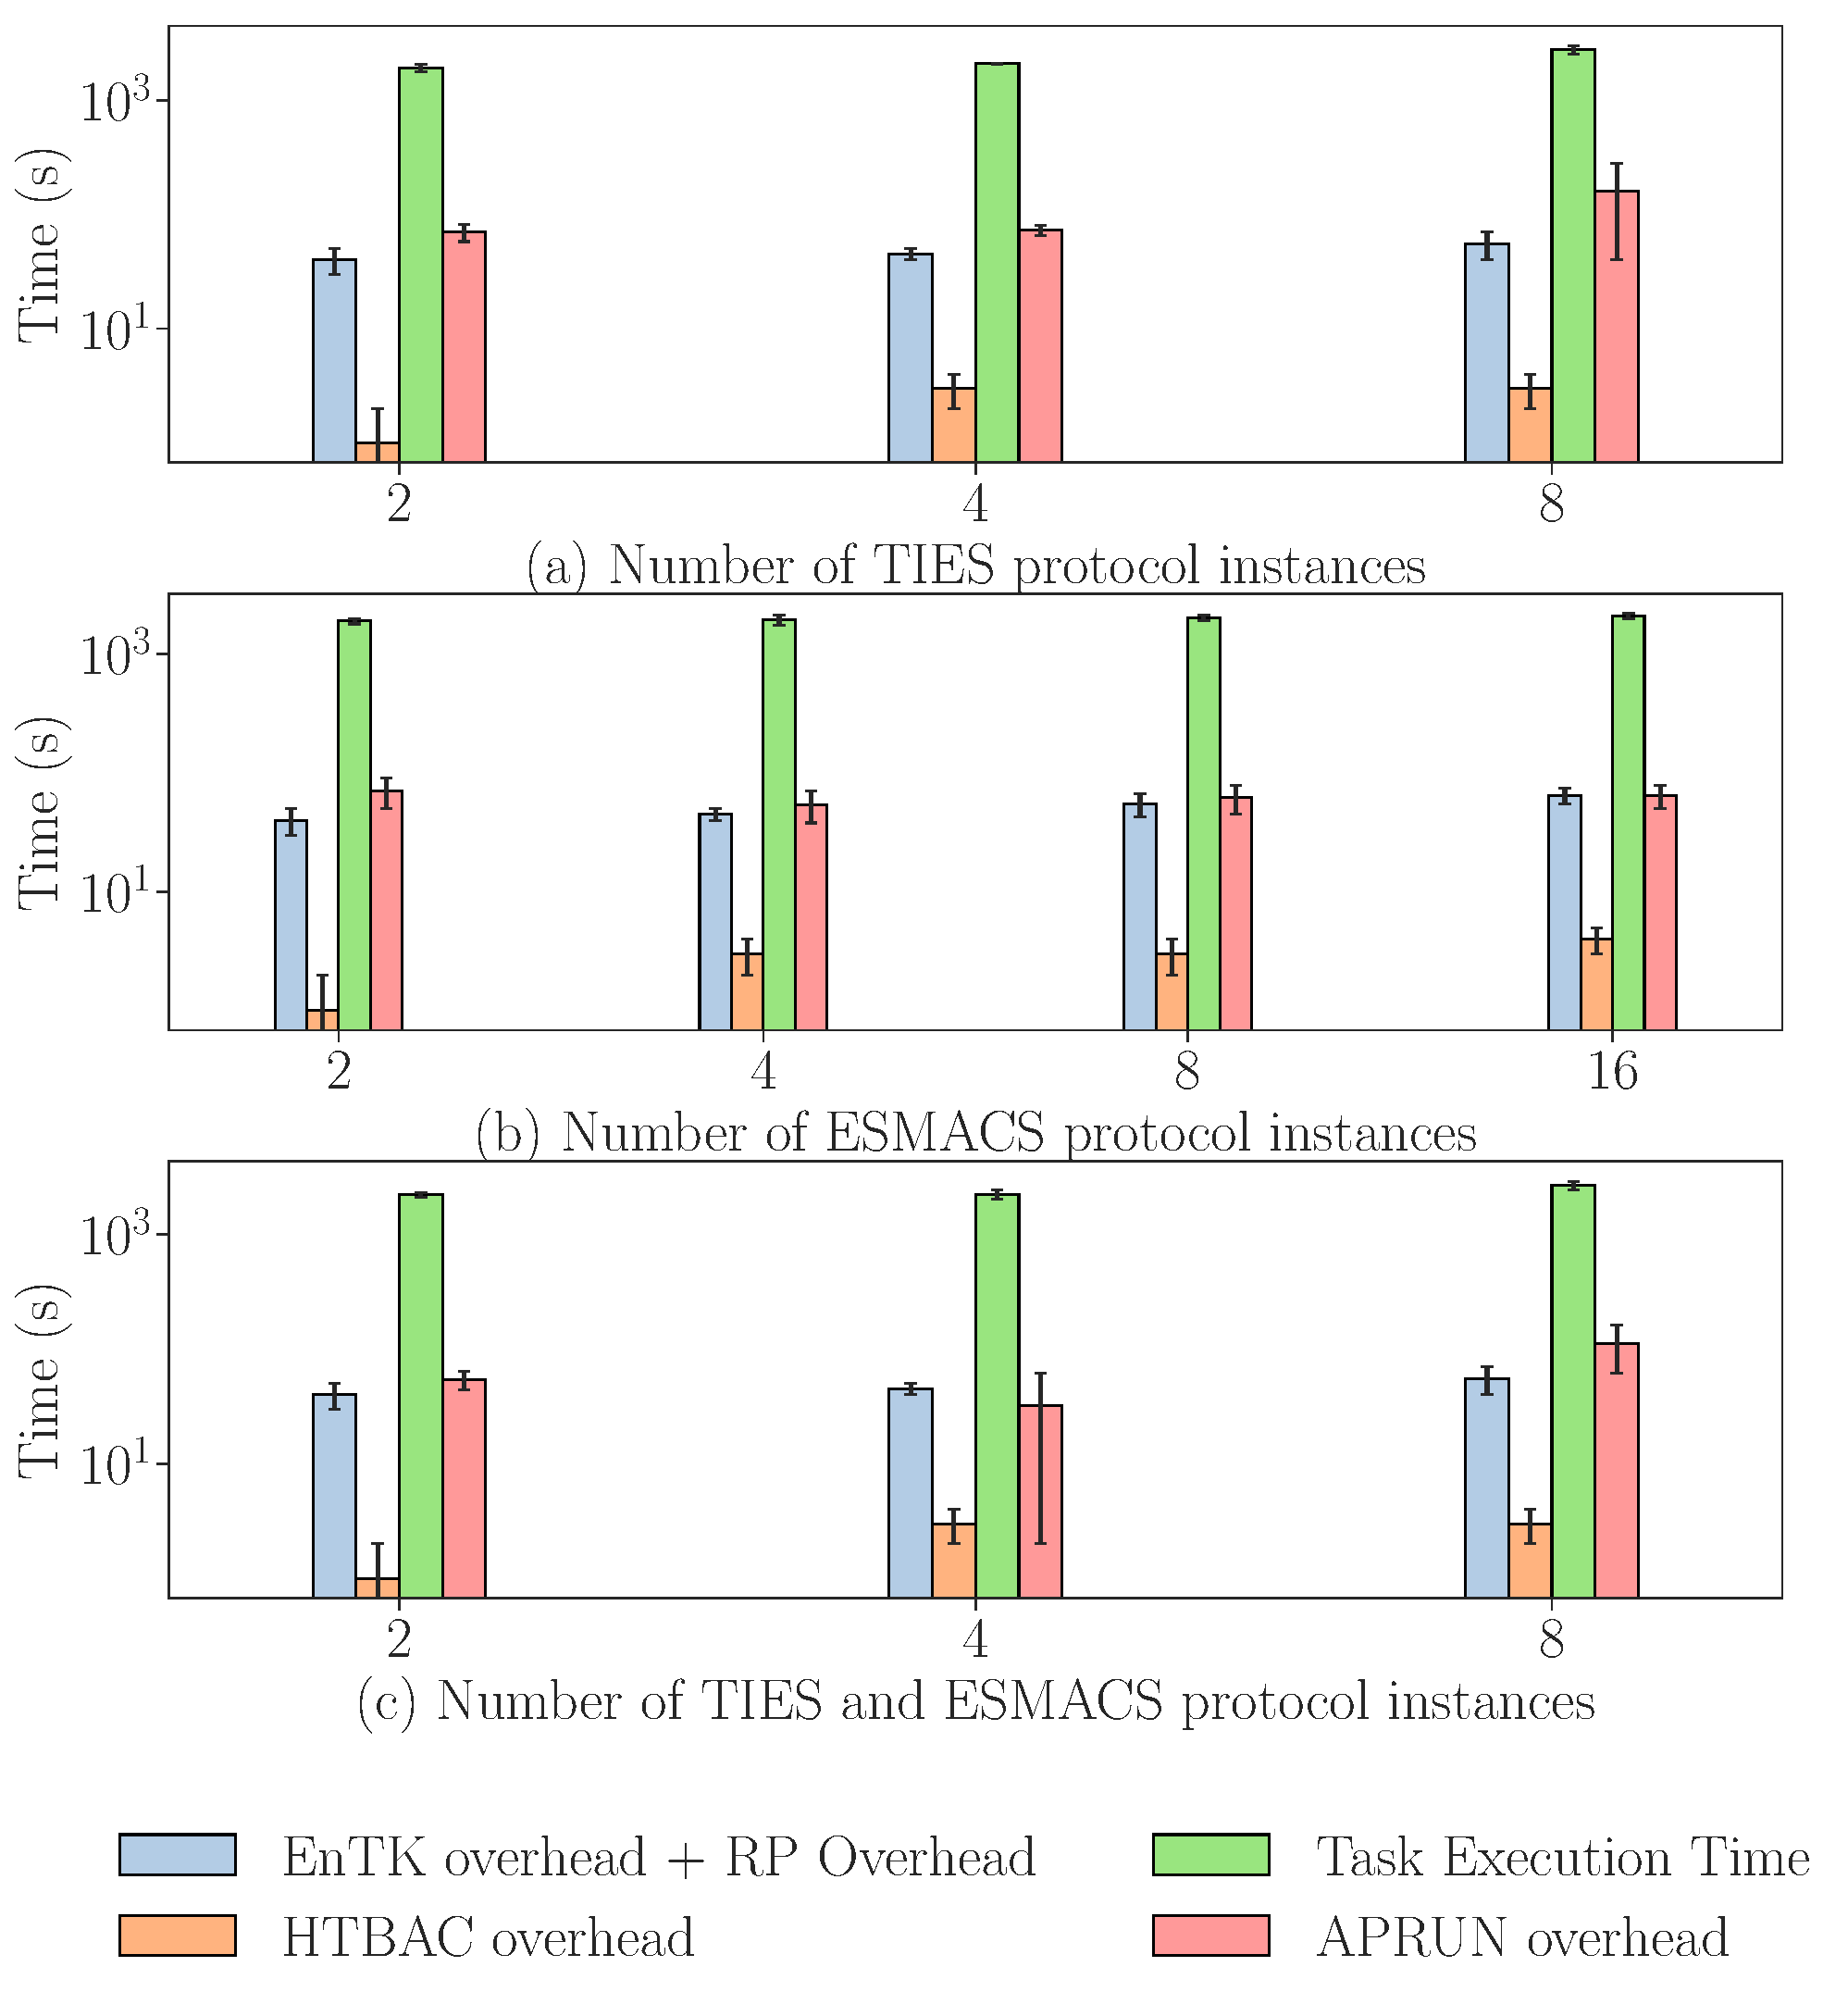
\includegraphics[width=\columnwidth]{figures/ws_all.pdf}
    \caption{Weak scaling properties of HTBAC. We
    investigate the weak scaling of HTBAC as the ratio of the number of
    protocol instances to resources is kept constant. Overheads of HTBAC, 
    EnTK + RP, and \texttt{aprun}, and \(TTX\) for experimental
    configurations investigating the weak scaling of TIES. We ran 3 trials
    for each protocol instance configuration.} 
\label{fig:ws}
\end{figure}

\jdnote{Maybe combine captions into 1?}\mtnote{Agreed.}\jdnote{One figure, 3 
subplots, 1 caption is cleaner}

The HTBAC overhead depends mostly on the number of protocol instances that
need to be generated for an application. This overhead shows a super linear
increase as we grow the number of protocol instances, but its duration is
negligible when compared to \(TTX\).
% HTBAC enables concurrent execution of multiple protocol \mtnote{what type
% of protocols?} instances.

\mtnote{I would create a subsection with overheads, discussing their behavior
and nature while referencing both weak and strong scaling experiments.}

The runtime overheads, mainly EnTK and RP, mostly depend on the number of
tasks that need to be translated in-memory from a Python object to a compute
unit (CU) description~\cite{dakka2017}. \mtnote{This sentence is copied from
a previous paper we wrote: does the reader know what a CU is?}
\jdnote{I will add in a brief mention of CU in Section IV}\mtnote{I would
just use task as you do in the following sentence. IMHO, using CU adds yet
another pseudo-technical term as a synonym of a term we are already using,
i.e., task}. As such, those overheads are expected to grow proportionally to
the number of tasks as observed in Figure\ldots, bar in \ldots color, \ldots.
\mtnote{Please add reference to the relevant figure(s) and details.} 

\mtnote{I commented all the following. IMHO, it does not contribute to
understand the current analysis of the results. Do we need to expand the
analysis?}
% ------------------------- COMMENTED BY MT -------------------------
% EnTK submits CU descriptions to a database that is then pulled by
% RP.\mtnote{I am not sure this is accurate}\jdnote{took out "same" database}
% In addition, each stage constructed by EnTK maintains sequential barriers.
% \mtnote{Doe the reader know what a barrier is?}\jdnote{I will add this to
% the EnTK description in Section IV} RP remains dormant until completion of
% the current tasks before staging the next tasks. \mtnote{This figure is
% about scaling behavior, not about the mechanics of EnTK and RP here
% discussed.}\jdnote{took out figure ref}
% ------------------------- END COMMENTED BY MT ----------------------

% The impact of the synchronization barriers increases with the number of CUs
% as seen in the 16 protocol instances data point in
% This pull operation occurs over a wide area networks, which introduces
% varying amounts of latency.

The RP overhead is calculated measuring and aggregating the execution time
(i.e., duration) of the RP components that manage and coordinate the
execution of the application. Among these components, the task scheduler of
RP introduces the largest overhead. The task scheduling overhead scales
linearly with the number of tasks because the time taken to schedule a task
depends on the total number of tasks that need to be scheduled. 
% The main contributor to the increase in overhead in RP is based on the the
% time of resources inactivity while RP schedules new tasks. As such, the
% overhead is expected to grow proportionally to the number of concurrent
% tasks~\cite{dakka2017}.
\mtnote{I am afraid this whole paragraph needed to be
rewritten. I tried to fix it but we are missing a comparative evaluation of
this overhead. For example, does this overhead matter when compared to TTX or
TTC? Given a computation campaign with TIES and ESMACS, how much allocation
time would be spent on this overhead? What would be the total percentage of
allocation/resources spent in overheads?}

% Among these durations, the pilot duration contains the time to bootstrap
% and terminate the pilot. The task overheads contain the executor's spawning
% of the task, folder staging preparation, and operating system task
% spawning. \mtnote{We need to explain to the reader why all this is relevant
% in this context.} \jdnote{need to discuss on 06/04, should we keep these
% details or keep the focus on the paragraph just above this one?}

Furthermore, an additional overhead, driven by the \texttt{aprun} launch
method increases as we approach a system limit on the number of concurrent
\texttt{aprun} processes. For example, when scaling to 8 TIES protocol
instances as shown in Figure~\ref{fig:weak_scaling_TIES}, the application
requires 520 concurrent tasks. Considering that we observe \texttt{aprun}
failures at approximately 436 concurrent processes, this accounts for
additional time that is factored into \(TTX\). \jdnote{add in the aprun
graph} \mtnote{We need to explain why TTX is affected. Are tasks restarted?
Also, does this overhead matter? See previous comment about RP overhead
impact on TTX/TTC/Resource utilization.}

% \mtnote{this sentence does not read well. I would refine it}
% \mtnote{this needs further explanation}
% \jdnote{reworded paragraph, also commented out next paragraph on EnTK
% synchronization until I can justify better.}

% \mtnote{Does the reader know what aprun is? Also, I would use something
% like textttt to identify the name of a command or
% executable}\jdnote{addressed}

% \mtnote{concurrent?}\jdnote{addressed} 

% Together, the EnTK-enabled synchronization barriers and \texttt{aprun}
% overhead failures \mtnote{until now, we have implicitly assumed that our
% overheads are measured in time. Did we now use also number of failures?}
% introduce delays in the scheduling of the CUs and results in higher
% overheads \mtnote{Is this sentence circular? Overhead increases
% contributing to increasing the overhead?}. Lastly, we notice that each
% additional protocol instance contributes to roughly 55 additional seconds
% in \(TTX\).\mtnote{All this needs to be clarified and expanded into an
% actual discussion of the results.}

% We use between 4160 and 16,640 cores as indicated in
% Figure~\ref{fig:weak_scaling_TIES}.

% To characterize the weak scaling performance of TIES \mtnote{I am not sure
% I understand this sentence: For measuring the weak scaling performance of
% TIES?}
% \jdnote{better?}, we use between 4160 and 33280 cores as indicated in
% Figure~\ref{fig:weak_scaling_TIES} because the NAMD executable used in all
% tasks \mtnote{does the reader know what a task is in this context?}
% \jdnote{will be defined in Section IV} from $S1$ -- $S4$ require
% \mtnote{grammar: requires} a single node i.e. 32 cores per task, as
% mentioned earlier in the APRUN limitation.
% \mtnote{why?}\jdnote{32 cores/task addressed by earlier mention of aprun
% MPI limit}

% With each new protocol instance generated for an application, the HTBAC
% overhead grows to match the additional requirement of generating new
% protocols.

% In order to understand the contribution of the various events in HTBAC,
% termed as HTBAC overhead, to

%----------------------------------------------------------------------------
% \subsubsection{Weak Scaling Experiments}

% We investigated the weak scalability properties for the TIES protocol by
% growing the number of protocol instances while adhering to the required
% number of pipelines. By design of each protocol, an increase in the number
% of instances simply means an increase in the number of pipelines. The first
% weak scalability experiment demonstrates the behavior of HTBAC, EnTK and RP
% using the multiple instances of the TIES protocol. By design of weak
% scaling, the ratio between the number of pipelines and cores are kept
% constant. As the number of cores (measure of resource) changes by a factor
% of 2, we introduce twice as many protocol instances. As designed, the weak
% scaling property provides insight into the size of the workload that can be
% investigated in a given amount of time.\mtnote{This paragraph is a copy of
% a previous paragraph. See comments and iterations of the previous paragraph
% before rewriting a new paragraph if needed.}

% ---------------------------------------------------------------------------
\subsection{Strong Scaling and Performance Characterization}

\mtnote{Should we have also a `Weak Scaling Experiments' header? Or maybe we
should change this one?}

To investigate strong scaling, we run two applications on Blue Waters: \ldots
and \ldots \mtnote{Please add name of the applications}. We investigate the
strong scaling behavior considering only homogeneous protocols. The
investigation of heterogeneous protocols is of interest but not at the risk
of cluttering the paper \mtnote{I am afraid we will need a better explanation
for this omission}. Both applications use the \texttt{BRD4-GSK} physical
systems \mtnote{Should this detail go in experiment design? This would apply
also to the weak scaling in the previous section}.

The first application \mtnote{name?} shows the strong scaling behavior of
TIES alone \mtnote{Are you sure this should not be the `nth experiment shows'
instead of the `first application shows'?}, using \texttt{NAMD-MPI} with 32
cores per task. We fix the number of instances of the TIES protocol to 8 due
to the described \texttt{aprun} limitations. We vary the amount of resources
between 4160, 8320 and 16640 cores. Given 4160 cores, we can execute 4
generations of 130 concurrent tasks; with 8320 cores, we can execute 2
generations of 260 concurrent tasks. The second application shows the strong
scaling behavior of the ESMACS protocol \mtnote{See previous comment about
application/experiment}. We fix the number of instances of the ESMACS
protocol to 16 and vary the amount of resources between 3200, 6400 and 12800
cores. This produces the same number of generations of execution \mtnote{add
reference to the subsection where generation is defined} as the first
application. \jdnote{will add the plot for ESMACS ss once I receive 2 full
trials}. As we increase the number of parallel resources,
Figure~\ref{fig:strong_scaling_TIES} shows linear speedup in \(TTX\) while
maintaining fixed $T_{O}$. The fixed $T_{O}$ suggests that the overheads are
mainly driven by the scheduling in the number of protocols and thereby the
number of tasks, not by the amount of resources. This is confirmed for RP in
Ref.~\cite{merzky2018}.\jdnote{I need to investigate this but I also presume
that aprun limits are also a factor of overhead.}

% The comparison between weak and strong scalability shows the overhead
% introduced by load balancing and scheduling tasks in multiple generations.

% By design of the TIES protocol, this workload show up to $65 \times 8$
% concurrent tasks, where each task uses 32 cores. The total number of
% concurrent

% \mtnote{See previous comments about terminology}\mtnote{I am not sure I
% understand: are we comparing overheads when weak and strong scaling our
% applications/workflows or are we first measuring the overheads when strong
% scaling and then comparing them to those of weak scaling?}. As we scale the
% number of generation of concurrent tasks executions, we half the resources
% allocated by the pilot \mtnote{this should be explained in the experiment
% setup and design}.

\mtnote{General note. Experiments about weak and strong scaling show the
behavior of our software stack with one or more workflows/workloads. The
question these experiments answer to is: Given a workload/workflow, does this
software stack scale weakly and/or strongly? This is why, in the analysis of
our data, we look at the linearity (or lack of thereof) of our plots. The
analysis of the overhead(s) answer to a different question: What part of a
measure---e.g., time to completion---depends on the properties of an element
used to produce that measure---e.g., a component of our software stack?
Usually, the analysis of the overheads is used to explain why we observe lack
of scalability (weak or strong) as represented by a superlinearity in our
plots. The discussion of our experimental results should clearly distinguish
these questions and properly relate the study of scalability to that of
overheads. At the moment, our discussion does not do all this.}\jdnote{I
reduced the discussion of scalability down to the properties that relate to
contributions of overheads and trends observed in TTX.}

\begin{figure}
  \centering
   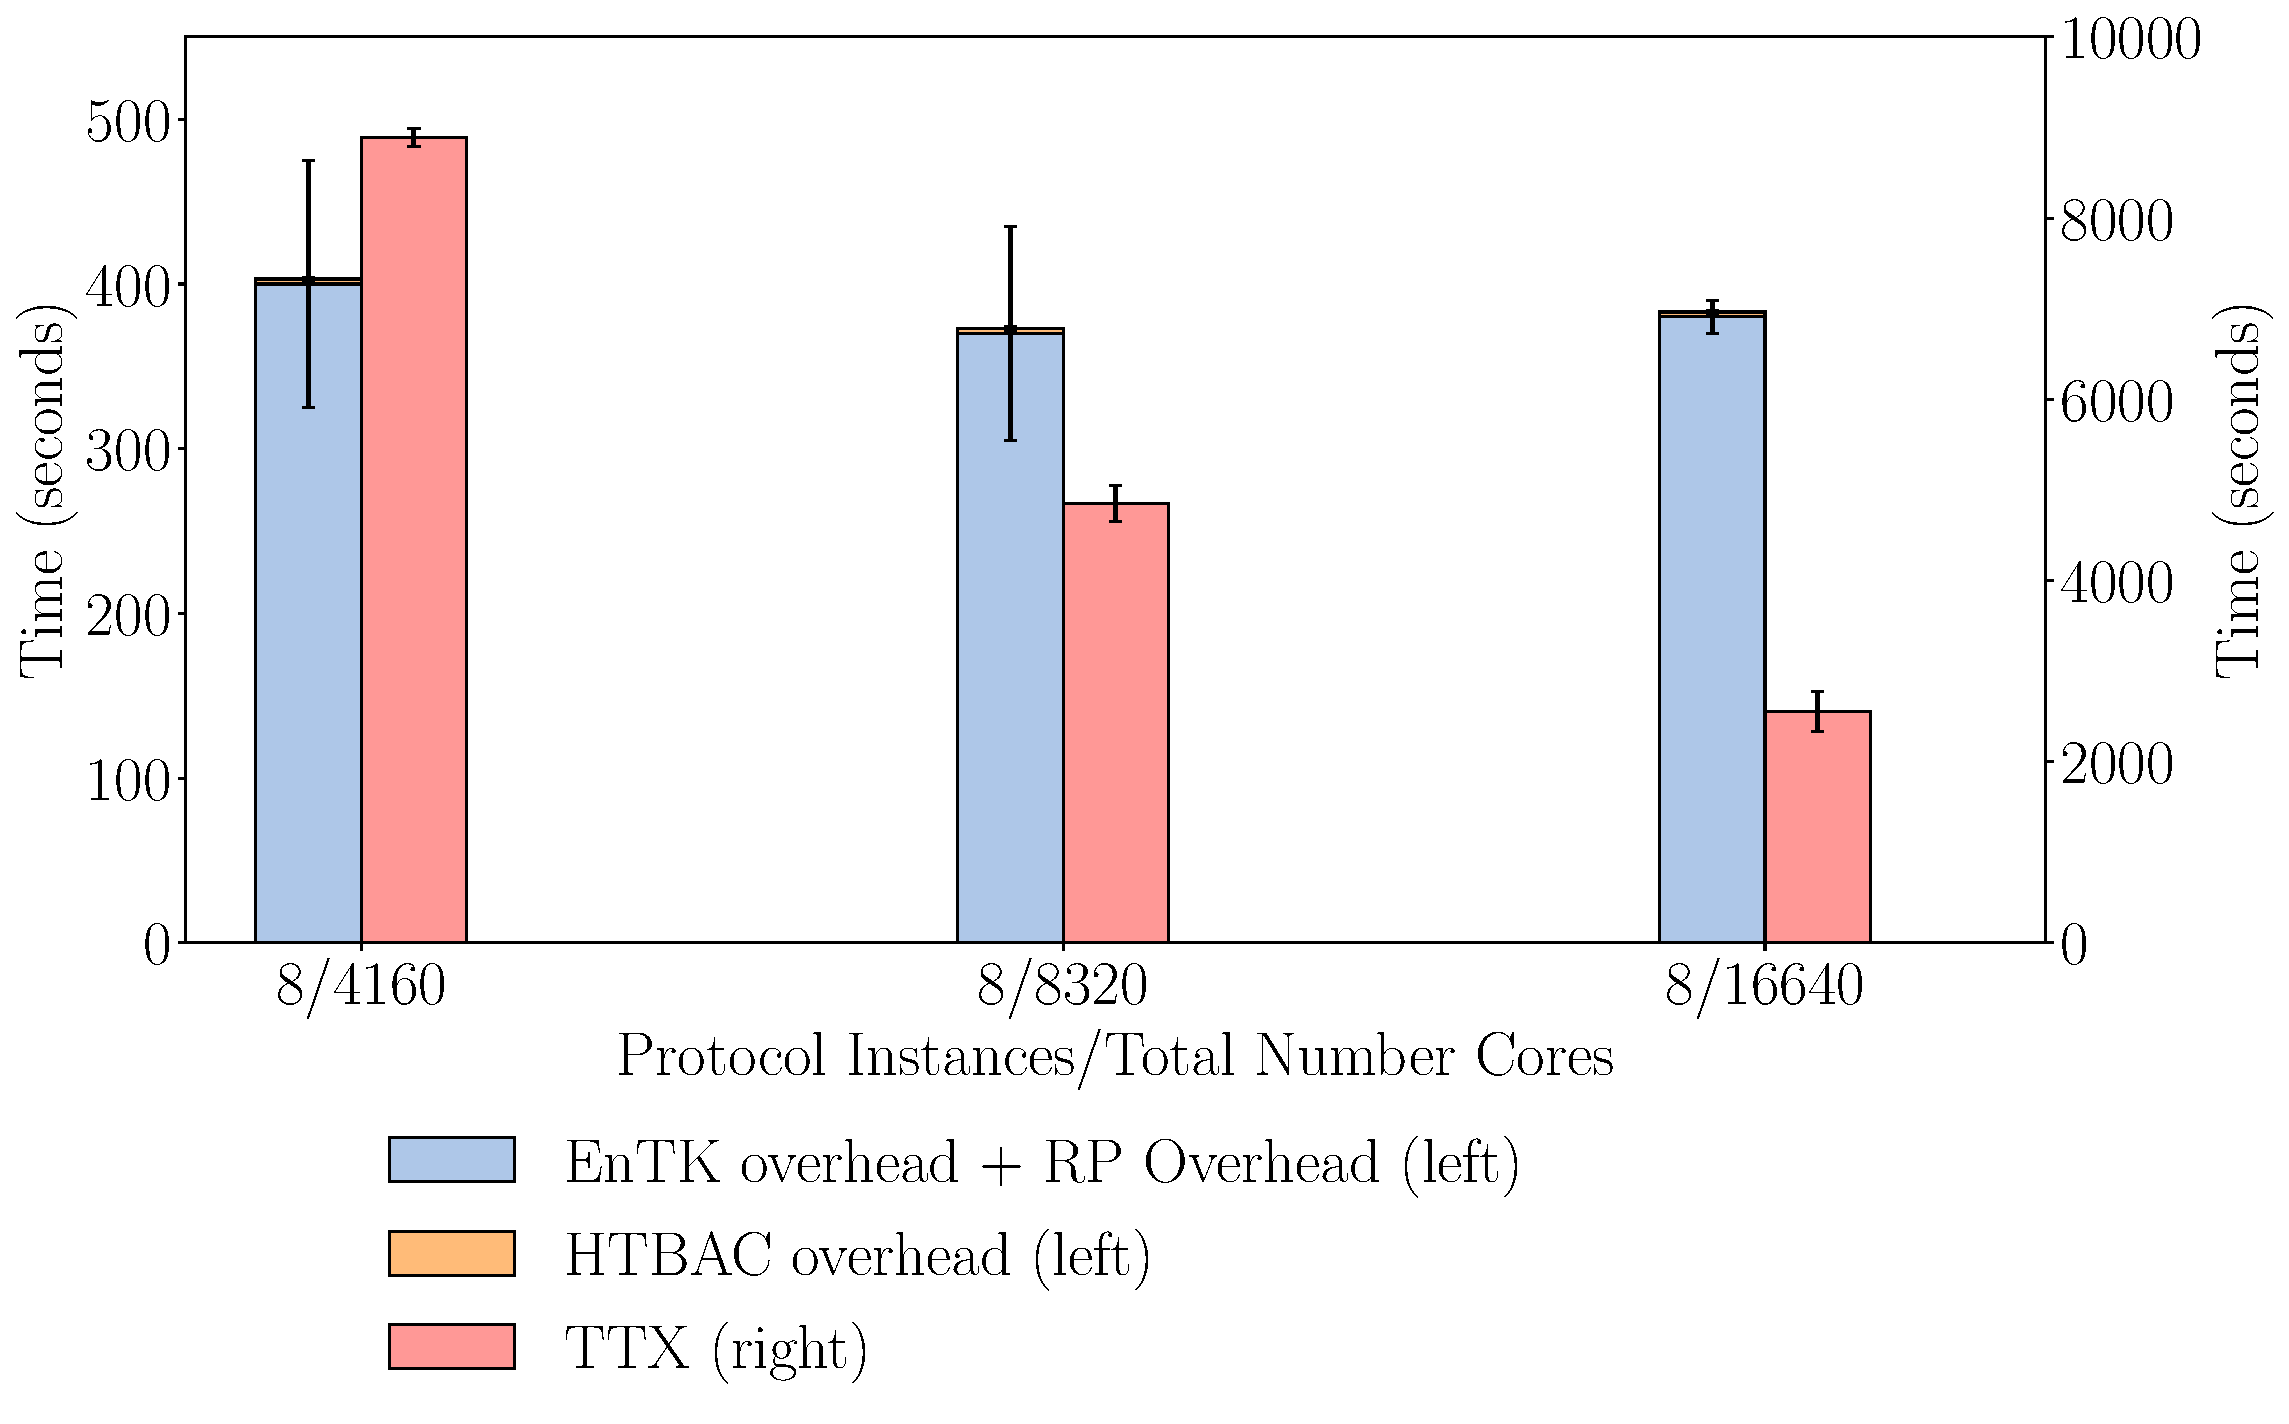
\includegraphics[width=\columnwidth]{figures/new_ss_ties.pdf}
    \caption{Strong scaling properties of HTBAC using TIES protocol. We
    investigate the strong scaling of HTBAC with a fixed number of protocol
    instances while varying the amount resources. Overheads of HTBAC and
    runtime overhead (left) and \(TTX\) (right) for experimental
    configurations investigating the strong scaling of TIES. We ran 3 trials
    for each configuration.}
\label{fig:strong_scaling_TIES}
\end{figure}



%----------------------------------------------------------------------------
\subsection{Experiments Validation}

% HTBAC automates the process of calculating the binding affinity of
% protein-ligand complexes from reading the input to analyzing the final
% results.

In order to validate the correctness of the results produced using HTBAC and
the BRD4-GSK physical systems, we compare our results with those previously
cited \mtnote{This is unclear. Do you mean: results that have been previously
published? If so, where?}. These experiments \mtnote{What experiments? The
previous sentence writes about a comparison.} are vital to gain confidence in
the algorithm \mtnote{which algorithm?} and to prove that it is indeed
calculating the correct values.

The validation experiments were based on the original study of Wan et
al.~\cite{Wan2017brd4} \mtnote{Note: `et al.' is an abbreviation of 'et
alia', Latin for `and [et] others [alia]'. As such, the correct spelling is
`et al.'. It is now corrected both here and in the table caption}. We
selected a subset of the protein ligand systems that were the subject of that
study: ligand transformations 3 to 1, 4, and 7. We then performed a full
simulation on all 3 systems and calculated the binding affinity using HTBAC.

The results of our experiments, collected in Table~\ref{tab:exp2}, show that
all three $\Delta \Delta$G values are within error bars of the original study
using the TIES protocol, reinforcing \mtnote{validating? Based on what we
wrote before this would seem to contradict our intent} the fact that the
results produced using HTBAC are indeed correct
\mtnote{I am not sure `correct' here applies to the results. We may want to
have a look about the difference between validation and verification,
focusing on the separation between methodology and results.}.

\begin{table}
  \centering
  \caption{Comparison of the calculated binding free energies using HTBAC,
  from the original study by Wan et al. and experimental data. In
  principle,\mtnote{Do they use the same protocol? If there are differences
  we should explain them.} the two theoretical studies used the same
  protocol. This experiment proved that HTBAC implemented TIES correctly, as
  the calculated values are either the same or within error bar of the
  original study. All values are in \textbf{kcal mol\textsuperscript{-1}}.}  
  % \begin{tabular}{l@{\hskip 1in}r@{\hskip 0.2in}r@{\hskip 0.2in}r}
  \begin{tabular}{lrrr}
    \toprule
    System & HTBAC & Wan et. al & Experiment \\
    \midrule
    BRD4 \textbf{3 to 1} & \num{0.39 +- 0.10} &   \num{0.41 +- 0.04} &  \num{0.3 +- 0.09} \\
    BRD4 \textbf{3 to 4} & \num{0.02 +- 0.12} &   \num{0.01 +- 0.06} &  \num{0.0 +- 0.13} \\
    BRD4 \textbf{3 to 7} & \num{-0.88 +- 0.17} &  \num{-0.90 +- 0.08} & \num{-1.3 +- 0.11} \\
    \bottomrule
  \end{tabular}
  \label{tab:exp2}
\end{table}

%----------------------------------------------------------------------------
% \subsection{Adaptive Experiments}

% The TIES workflow can benefit from an adaptive execution environment to
% improve the efficiency and accuracy of result. In \emph{adaptive
% experiments} we implemented the adaptive quadrature algorithm specifically
% customized for biosimulations.

% In the adaptive workflow, we alter the number of $\lambda$ windows being
% simulated over the course of a protocol instance. The position of new
% $\lambda$ windows depends on the estimated error of the integral measured
% between adjacent windows. Increasing the number of $\lambda$ windows in
% regions of rapid change will increase the accuracy of the overall integral
% to a greater degree than an arbitrarily placed window. In order to
% adaptively add lambda windows, we need access to the $\partial
% U/\partial\lambda$ values during runtime. Therefore, we break down the
% single production simulation stage (S4) \mtnote{I would reference the
% figure with the workflow diagram here} from the nonadaptive workflow into
% multiple smaller stages \mtnote{how many?}, each running for 1 ns. Once
% each simulation is complete within a stage, a decision is made about
% whether more $\lambda$ windows are required, and, if so, where these
% windows should be placed.

% We start out the simulation with 5 replicas of 3 \mtnote{why emphasis for
% 3?}\jdnote{addressed} equally spaced $\lambda$ windows, and equilibrate
% them. Then we repeatedly execute shorter production simulations followed by
% an analysis phase which determines where to place new lambda windows. This
% procedure is repeated until convergence, at which point all concurrent
% simulation are terminated. We define convergence as the point in the
% production-analysis loop at which a desired error threshold is reached.

% The success of this algorithm is determined by the decision where
% additional $\lambda$ windows should be introduced. In adaptive quadrature,
% this decision is made by calculating an error estimate on the integral and
% comparing this estimate to a threshold value. Due to the stochastic nature
% of biosimulations, it is non-trivial to determine this error and, as a
% proof of concept, we simplified this decision to replicate pre-calculated
% results. In future studies, we plan to use a dynamic decision process.

% Inter-node communication introduces a constraint on the number of new
% $\lambda$ windows that can be added at each iteration. Simulations must run
% on an integer number of nodes to reduce the overhead of inter-node
% communication. This means that the number of new $\lambda$ windows (i.e.,
% the number of simulations) \emph{has} to be either doubled or left
% unchanged. If the number of windows is doubled, the number of nodes per
% simulation can be halved automatically. Our algorithm loops through the
% current $\lambda$ window pairs until this criterion is reached, forcefully
% adding more windows when needed.


% I don't think we need this equation here, it's too trivial.
% \begin{flalign} L &= \{ x_i: x_i\in[0,1]\; and\; x_{i+1} = x_i + \delta \},
% where\ \delta\ is\ 0.5. %&$$L=\{ x_i: x_i\in[0,1]\; and\; x_{i+1} = x_i +
% \delta \}$$%, where $\delta$ is $0.1$.
% \end{flalign}

% For every $\lambda$ window we initialize with five replicas therefore
% yielding a total of 15 tasks. We run 15 tasks for stages $S1$ through
% $S4.1$. Between stages $S4.1$ and $S4.3$ the number of $\lambda$ windows
% doubles for every stage, which doubles the total number of tasks. The last
% production simulation stage, $S4.4$, runs for the remaining 2 ns durations.

% Our experiments implement adaptive change in the $\lambda$ windows sampled
% and not the timing of execution. In this way, we introduce only a single
% \mtnote{additional?} degree of freedom relative to \mtnote{compared to?}
% our baseline ``non-adaptive" experiments. HTBAC provides the functional
% capability to adaptively determine the time at which the $\lambda$ windows
% are chosen. However, in this paper we do not investigate the impact of such
% adaptivity, as the objective is to determine the feasibility of adaptive
% execution and the scientific merit of adaptive decision making.

%----------------------------------------------------------------------------


% \begin{figure}
%   \centering
%     \includegraphics[width=\columnwidth]{figures/adaptive_vs_nonadaptive_ps
%     eudo.pdf}
%     \caption{Illustrating the adaptive vs. non-adaptive workflow given the
%     same number of core hours}
% \label{fig:adaptive_vs_nonadaptive_TIES}
% \end{figure}

% ---------------------------------------------------------------------------
\subsection{Adaptive Experiments}

\mtnote{Should this be Results as a whole? Or are we missing the results for all
the others?} \kfnote{I think results and experiments are one section. This
subsubsection is for the adaptive quadrature. There is a separate one for
adaptive termination.}\mtnote{I agree and both approaches would work for me. We
may want to be consistent across all experiments though: either we use a single
subsection illustrating the results of all the experiment or we discuss the
result of each experiment as we introduce it.} \kfnote{Okay. We are going
with the second approach. Describe experiment then results in the same
subsection.}

The aim of introducing adaptive quadrature to alchemical free energy
calculation protocols (e.g. TIES) is to reduce time to completion while
maintaining (or increasing) the accuracy of the results. Time to completion
is measured by the number of core hours consumed by the simulations. Accuracy
is defined as the error with respect to a reference value, calculated via a
dense $\lambda$ window spacing (65 windows). This reference value is used to
establish the accuracy of the non-adaptive protocol (which has 13 $\lambda$
windows) and the adaptive protocol (which has a variable number of $\lambda$
windows, determined at run time).

One of the input parameters of the adaptive quadrature algorithm is the
desired acceptable error threshold of the estimated integral. We set this
threshold to the error of the non-adaptive algorithm calculated via the
reference value. The algorithm then tries to minimize the number of $\lambda$
windows constrained by the accuracy requirement.

Table~\ref{tab:adapquad} shows the results of running adaptive quadrature on 5
protein ligand systems, comparing the \(TTX\) and accuracy versus the
non-adaptive case. The number of lambda windows are reduced on average by
\SI{32}{\percent}, hence reducing \(TTX\) by the same amount. The error on the
adaptive results is also decreased, on average by \SI{77}{\percent}. More
importantly, the error on all of the systems are reduced to below \num{0.2}
kcal/mol, which has recently been shown \cite{} to be the upper bound of
reproducibility across different MD engines. 

The TTX of the TYK2 L7-L8 system has increased for the adaptive run by 1
$\lambda$ window compared to the non-adaptive case. This is due to the
non-adaptive error begin very low, and matching that same accuracy required the
use of a large number of windows. Nonetheless due to the efficient placing of
the windows, the accuracy of the free energy still increased by
\SI{40}{\percent}.

\begin{table*}
  \caption{Comparing results of adaptive, non-adaptive and reference runs}
  \label{tab:adapquad}
  \begin{tabular}{lSSSSSS}
    \toprule
    {System}                               & 
    {Ref $\Delta \Delta$G}                 &
    {Non-adaptive $\Delta \Delta$G}        &
    {Adaptive $\Delta \Delta$G}            &
    {Num. of $\lambda$ windows}            &
    {Decrease in time to completion}       &
    {Increase in accuracy}                 \\
    \midrule
    {PTP1B L1-L2}   & 
    -58.51 & 
    -57.87(64) & 
    -58.60(9) & 
    10 & 
    \SI{23}{\percent} & 
    \SI{86}{\percent} \\
    %
    {PTP1B L10-L12} & 
    1.83   & 
    2.05(22) & 
    1.94(7)  & 
    6  & 
    \SI{54}{\percent} &
    \SI{68}{\percent} \\
    %
    {MCL1  L32-L38} & 
    2.13   & 
    2.33(20) & 
    2.14(1)      & 
    7  & 
    \SI{46}{\percent} & 
    \SI{95}{\percent} \\
    %
    {TYK2  L4-L9}   &
    -28.69 & 
    -28.25(44) & 
    -28.67(1)  & 
    7  & 
    \SI{46}{\percent} & 
    \SI{98}{\percent} \\
    %
    {TYK2  L7-L8}   & 
    4.97   & 
    4.92(5) & 
    5.00(3)      & 
    14 &  
    \SI{-8}{\percent} & 
    \SI{40}{\percent} \\
    \bottomrule 
    
  \end{tabular}
\end{table*}

Figure~\ref{fig:adapconv} \mtnote{missing figure? There is a table with the
label `adapquad' but not a figure.} \kfnote{Fixed} shows progression of the
algorithm, starting from 3 initial lambda windows, and at each iteration
bisecting the interval where the error is above the set threshold. For system X,
we can see as how the parts of the function that change less have relatively
fewer windows, while parts of greater change (usually, though not always around
the $\lambda=0.5$ mark) have more $\lambda$ windows to represent the shape of
the function more closely.

\kfnote{Move this to algorithm description} In previous studies \cite{} the
error estimation during the adaptive algorithm is done by calculating the
integral estimate using two methods, one lower and one higher in complexity,
then the difference between the two can constitute as a rough estimate of the
error on that interval.

\begin{figure}
  \begin{tikzpicture}
\begin{axis}[
  title style={align=center},
  title={Observed accuracy of adaptive vs. non-adaptive workflows\\for same simulation duration ({\SI{6}{\nano\second}}) },
  no markers,
  every axis plot/.append style={ultra thick},
  xlabel=Resource consumption (CPU-hours),
  ylabel=Error (kcal/mol),
  scaled ticks=false,
  yticklabel style={
  /pgf/number format/precision=3,
  /pgf/number format/fixed},
  scale=0.85,
  ]
  
  
\addplot+[color=Orchid, smooth] table [x=Resource consumption, y=Non-adaptive error, col sep=comma] {figures/non_adaptive_accuracy.csv};

\addplot+[color=YellowGreen, smooth] table [x=Resource consumption, y=Adaptive error, col sep=comma] {figures/adaptive_accuracy.csv};

\legend{Non-adaptive,Adaptive}

\draw[densely dotted, color=gray] (10586.058921984,0.049299384672436553) -- (12000,0.049299384672436553);
\draw[densely dotted, color=gray] (8143.1222476800012,0.0015858767437348931) -- (12000,0.0015858767437348931);

\draw[densely dotted, color=gray] (10586.058921984,0.08) -- (10586.058921984,-0.025);
\draw[densely dotted, color=gray] (8143.1222476800012,0.08) -- (8143.1222476800012,-0.025);
\draw[->] (10586.058921984,0.075) -- (8143.1222476800012,0.075) ;
\node[align = right] at (8700, 0.115) {Resource\\consumption\\decrease};

\node at (9200, 0.025) {\contour{white}{Error decrease}};
\draw[->] (11500,0.049299384672436553) -- (11500,0.0015858767437348931) ;


  
\end{axis}
\end{tikzpicture}

  \caption{\sout{This is a good plot!} Please provide a meaningful caption}
  \label{fig:adapconv}
\end{figure}

\begin{figure*}
  \begin{tikzpicture}
\begin{axis}[
  ybar,
  ymin=0,
  ylabel=Error (kcal/mol),
  x tick label style  = {text width=1.5cm,align=center},
  symbolic x coords={PTP1B L1-L2,PTP1B L10-L12,TYK2 L7-L8,TYK2 L4-L9,MCL1 L32-L38}
  ]
  
\addplot+[color=Orchid] table [x=System, y=Non-adaptive error, col sep=comma] {figures/savings.csv};

\addplot+[color=YellowGreen] table [x=System, y=Adaptive error, col sep=comma] {figures/savings.csv};


\legend{Non-adaptive,Adaptive}
  
\end{axis}
\end{tikzpicture}%
%
%
\begin{tikzpicture}
\begin{axis}[
  ybar,
  ymin=0,
  ylabel=Resource consumption (CPU-hours),
  x tick label style  = {text width=1.5cm,align=center},
  symbolic x coords={PTP1B L1-L2,PTP1B L10-L12,TYK2 L7-L8,TYK2 L4-L9,MCL1 L32-L38}
  ]
  
\addplot+[color=Orchid] table [x=System, y=Non-adaptive cpuh, col sep=comma] {figures/savings.csv};

\addplot+[color=YellowGreen] table [x=System, y=Adaptive cpuh, col sep=comma] {figures/savings.csv};


\legend{Non-adaptive,Adaptive}
  
\end{axis}
\end{tikzpicture}

\caption{\sout{This is a good plot!} Please provide a meaningful caption}
  \label{fig:savings}
\end{figure*}
